\documentclass[twoside, 11pt, a4paper]{article}

% --- 载入样式与宏包 ---
% 将所有的 \usepackage 和格式定义放在 cls/my_thesis_style.cls 中
\usepackage{cls/my_thesis_style} 

\begin{document}

% --- 2. 封面 ---
\begin{titlepage}
    \pagenumbering{gobble}
    \vspace*{\fill}
    \begin{center}
        {\sanhao\bfseries 硕士学位论文题目 \par}
        \vspace{2em}
        {\sihao Technical Artist \par}
        \vspace{1em}
        {\sihao \today \par}
    \end{center}
    \vspace*{\fill}
\end{titlepage}

% --- 3. 前言部分 (摘要、目录) ---
\cleardoublepage
\pagenumbering{Roman}
% 中文摘要
\phantomsection
\addcontentsline{toc}{section}{摘要}
\begin{center}
    {\xiaosan\songti 摘\qquad 要}
\end{center}
\vspace{1em}
本文档内容主要涵盖了二次元（NPR）渲染核心...（此处省略原文内容）

\vspace{1em}
\noindent {\wuhao\textbf{关键词：}} {\wuhao\songti 渲染管线\quad 材质Shader\quad 性能优化}

\cleardoublepage

% 英文摘要
\pagenumbering{roman}
\phantomsection
\begin{center}
    {\sihao\bfseries ABSTRACT} 
\end{center}
\addcontentsline{toc}{section}{\protect\rmfamily\bfseries ABSTRACT}

\vspace{1em}
\xiaosi The content of this document...（此处省略原文内容）

\vspace{1em}
\noindent {\xiaosi\bfseries KEYWORDS:} {\xiaosi Rendering Pipeline; Shader Material; Performance Optimization}

% 本模板中目录仅展示到三级标题，且一级标题会显示为“第X章”，
% 请根据需要调整 cls/my_thesis_style.cls 中的相关设置
\cleardoublepage
\markboth{目\qquad 录}{目\qquad 录}
\fancyhead[EC]{\headerfont 目\quad 录}
\tableofcontents
\cleardoublepage
\fancyhead[EC]{\headerfont \leftmark}

% --- 4. 正文部分 ---
\pagenumbering{arabic}
% 下句为示例，编译正式内容时请保持注释或删除
% % 主要包括各种内容的语法示例，如各级标题、图片、表格、公式等
\section{二次元核心渲染}    % 一级标题示例

\subsection{核心渲染算法}   % 二级标题示例
下面是个图片示例如图\ref{fig:1-1}所示\cite{2}。如表\ref{tab:1-1}所示\cite{1}。

% 图片和表格示例
\begin{figure}[htbp]
    \centering
    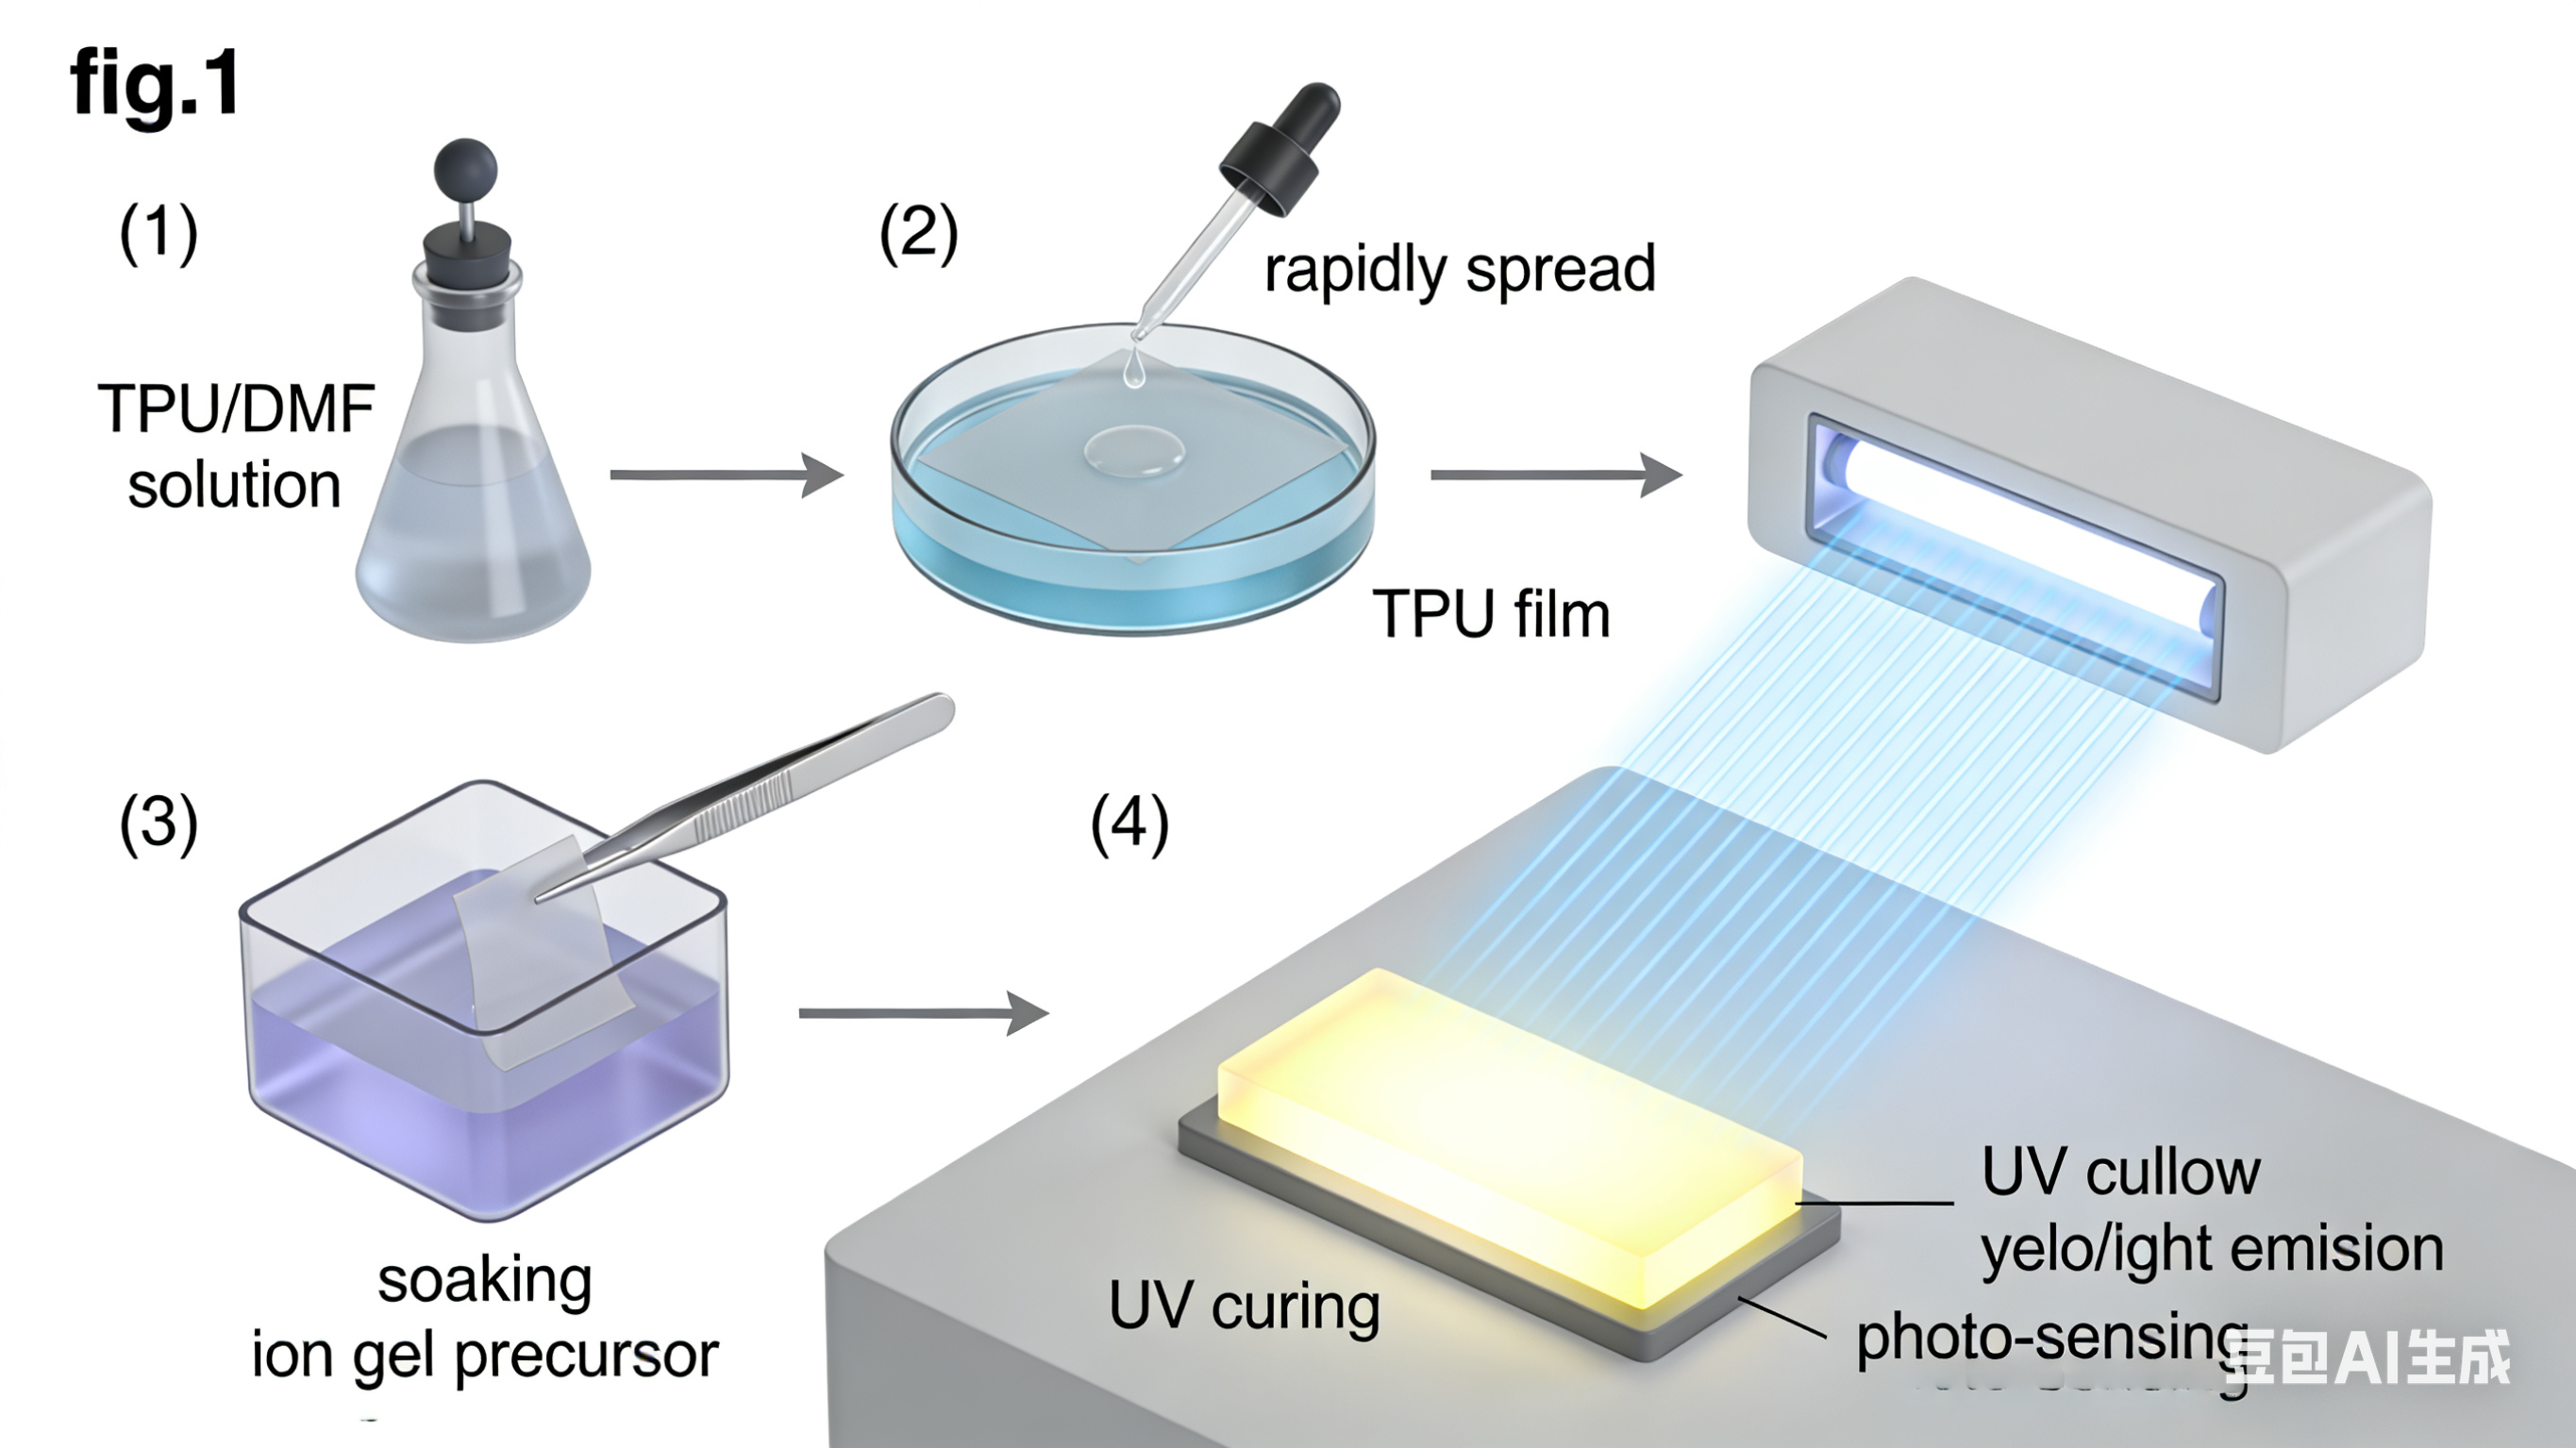
\includegraphics[width=0.8\textwidth]{fig/1-1.png} 
    \bicaption{渲染管线流程图}{Flowchart of rendering pipeline}
    \label{fig:1-1}
\end{figure}

\subsection{描边方案}
\begin{table}[htbp]
    \centering
    \bicaption{Unity 常用渲染路径性能对比}{Performance comparison...}
    \begin{tabular}{@{} lcc @{}}
        \toprule
        渲染路径 & 动态光源支持 & 内存开销 \\
        \midrule
        前向渲染 & 较少 & 低 \\
        \bottomrule
    \end{tabular}
    \label{tab:1-1}
\end{table}

\section{二次元核心渲染}

\subsection{仿生突触器件概述}
下面是个图片示例：\cite{1}

\begin{figure}[htbp]
    \centering
    % 注意：路径已经包含了 figures/
    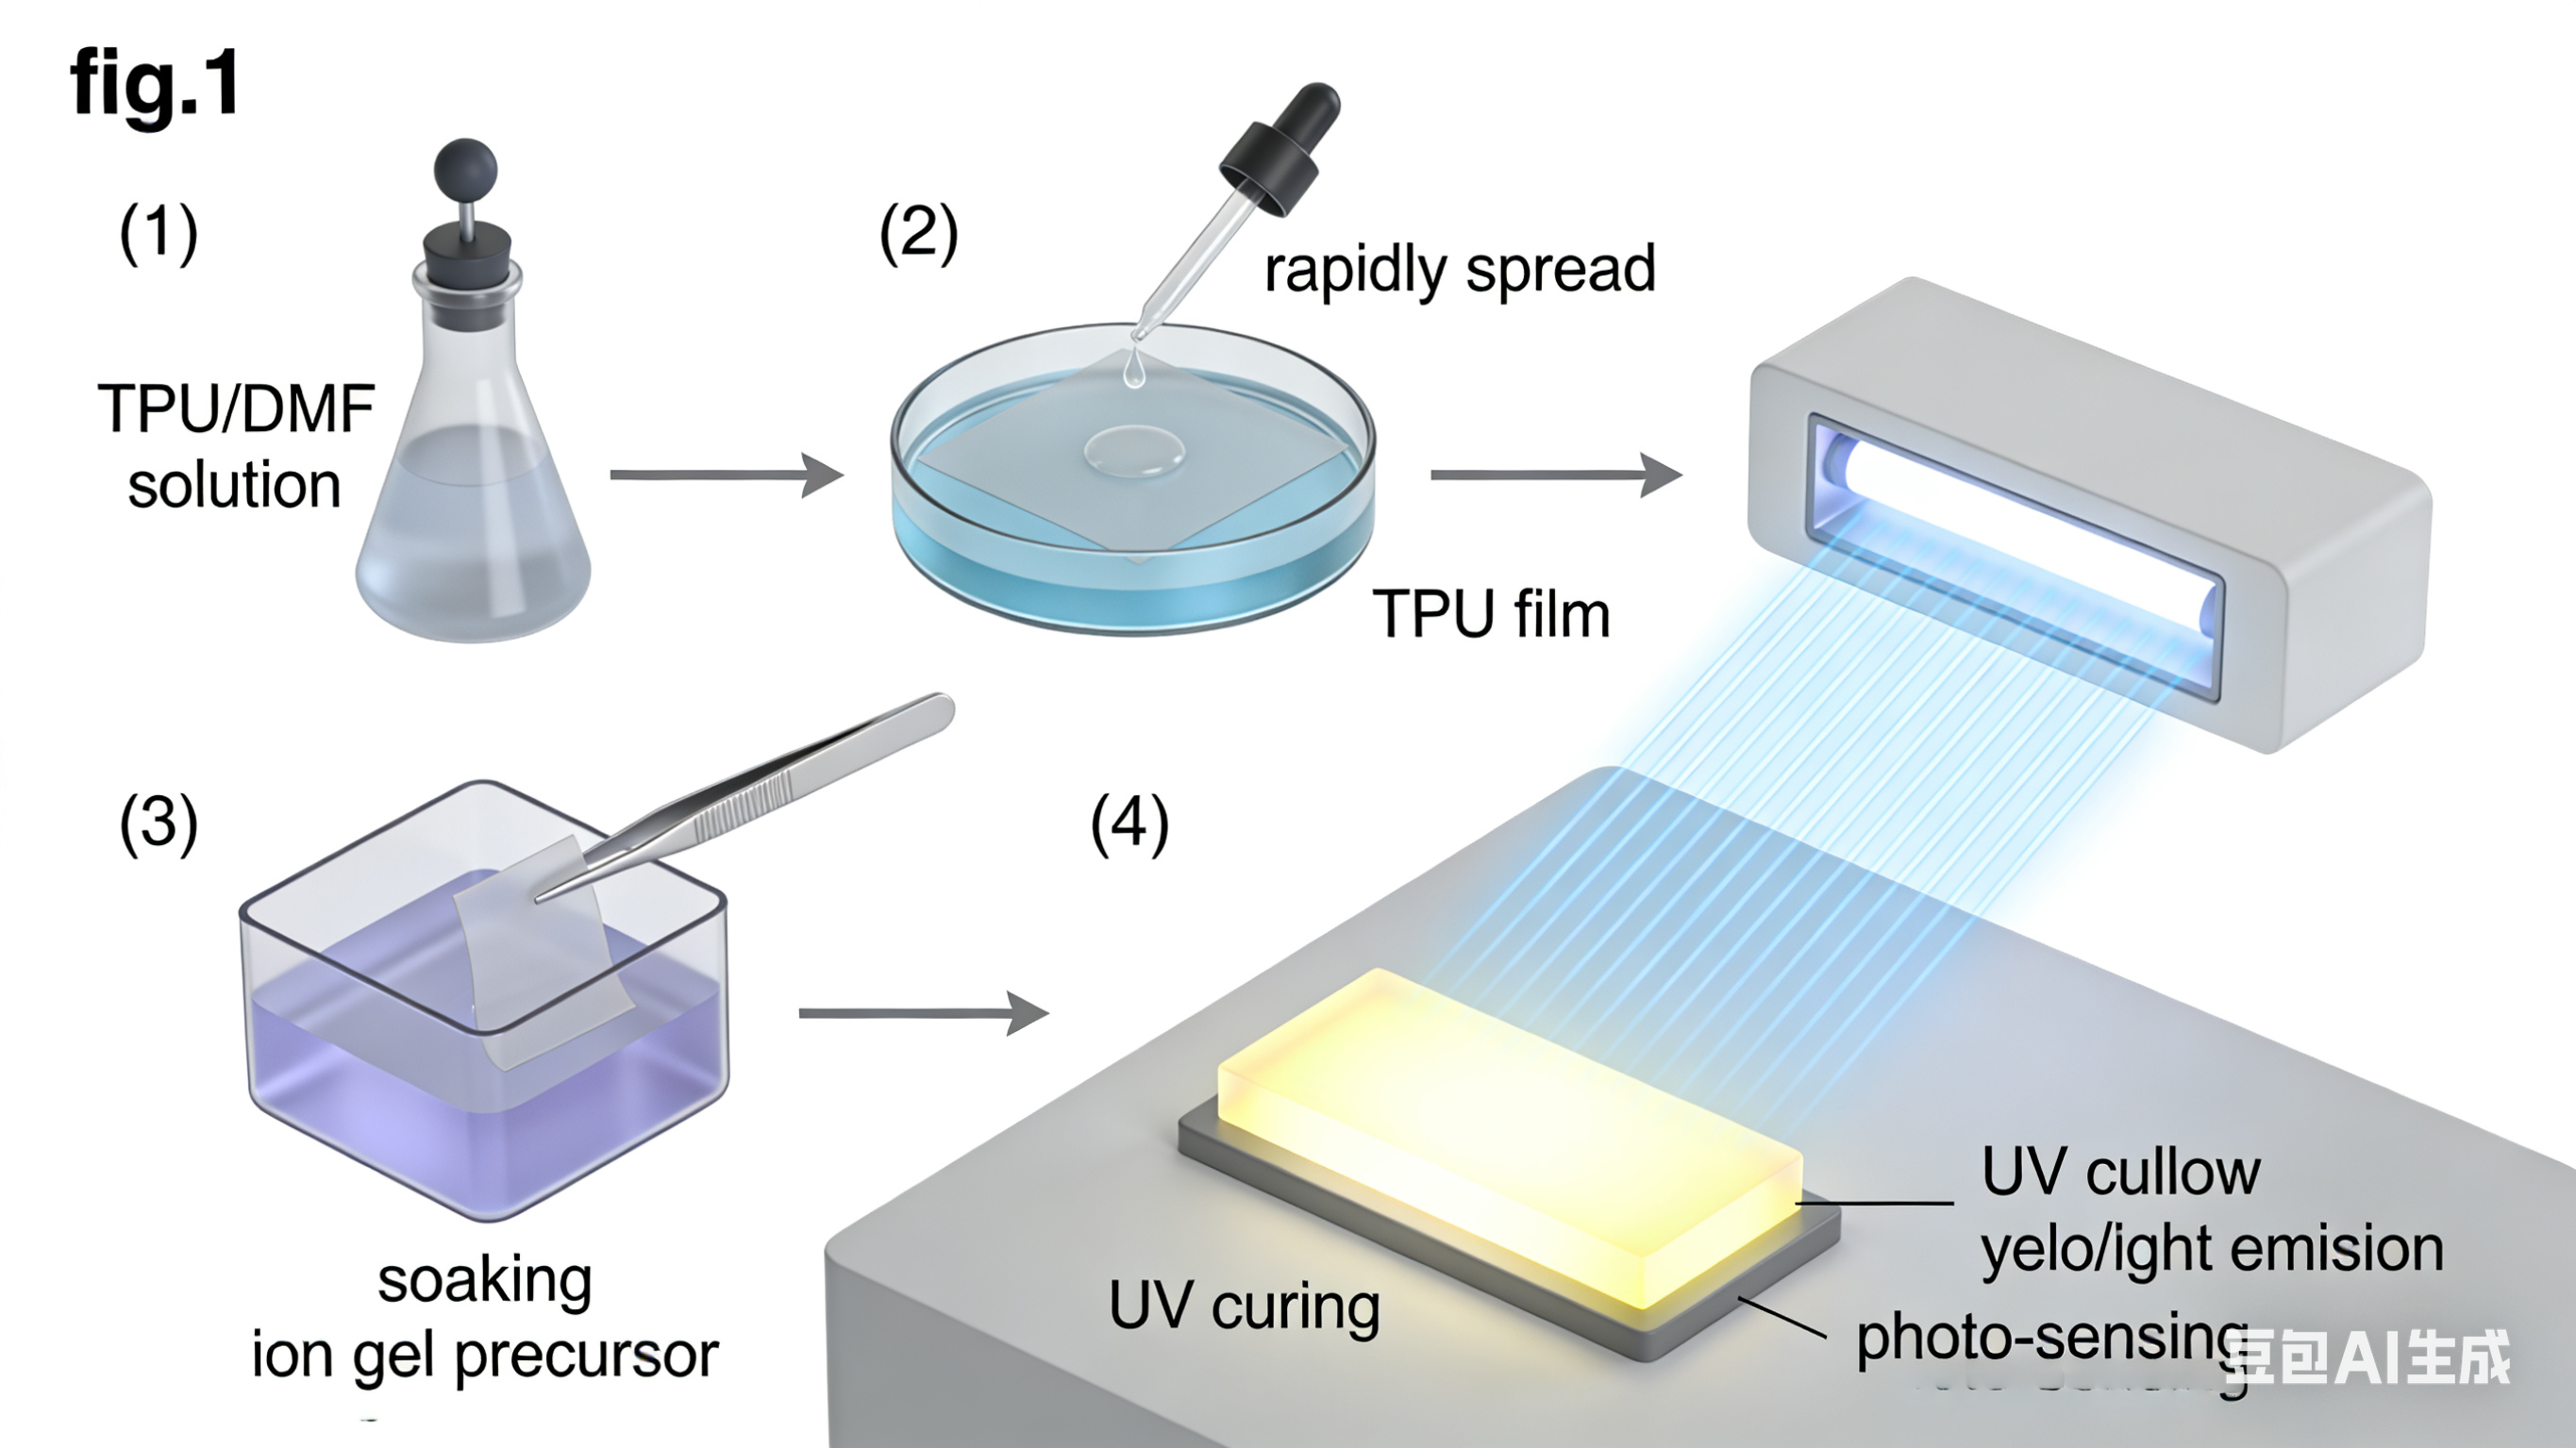
\includegraphics[width=0.8\textwidth]{fig/1-1.png} 
    \bicaption{渲染管线流程图}{Flowchart of rendering pipeline}
\end{figure}

\subsection{性能对比}
\begin{table}[htbp]
    \centering
    \bicaption{Unity 常用渲染路径性能对比}{Performance comparison...}
    \begin{tabular}{@{} lcc @{}}
        \toprule
        渲染路径 & 动态光源支持 & 内存开销 \\
        \midrule
        前向渲染 & 较少 & 低 \\
        \bottomrule
    \end{tabular}
\end{table}



% --- 5. 参考文献 ---
\newpage
\phantomsection
% 这里只用这一行，绝对不要再写 \bibliographystyle
\printbibliography[heading=bibintoc, title={参考文献}]

\end{document}